\indent\indent The top part of the grid creation tool offers different means to create a grid for your analysis. It also displays information and parameters which will be used in the correlation process.

\begin{figure}[!h]
   \centering
   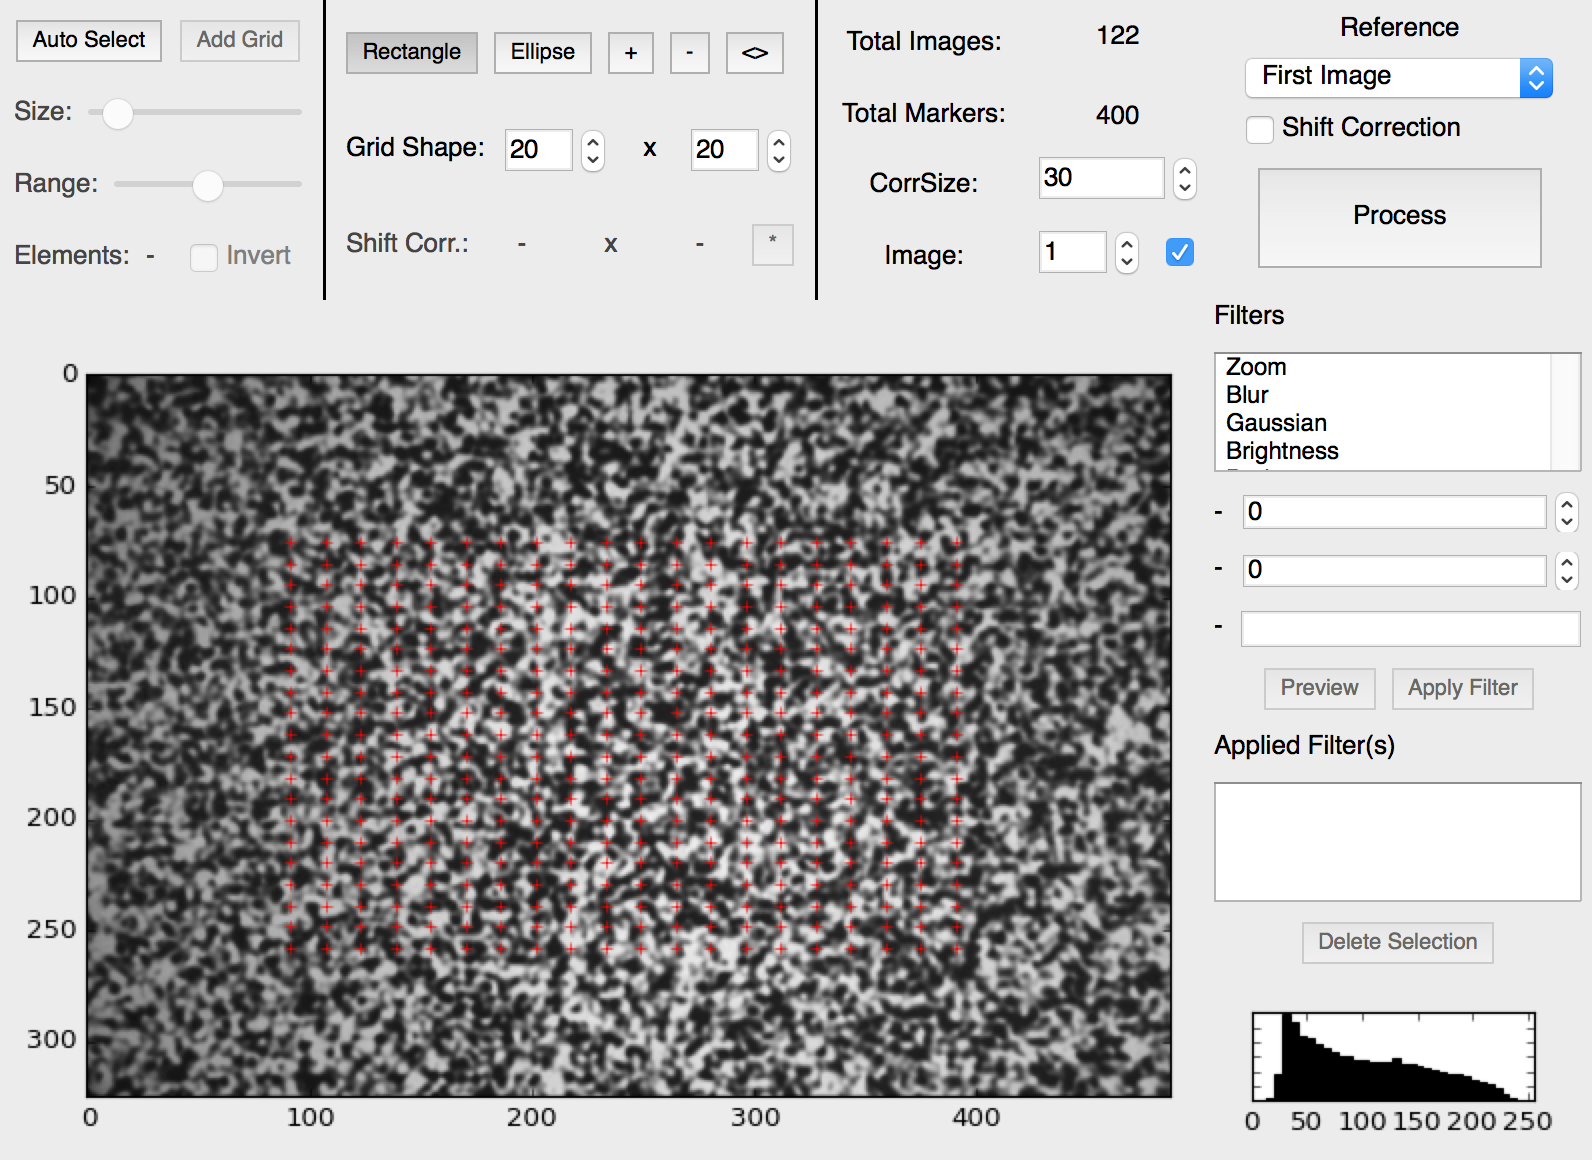
\includegraphics[scale=.4]{grid_creation}
   \caption{New Analysis: Grid Definition}
\end{figure}

\paragraph{Grid Creation\\\newline}
\label{par:Grid Creation}
\indent In order to run an analysis, a grid have to be defined. A grid is a set of markers with different coordinates which constitute the base of the correlation. When the images will be processed, the algorithm will track each marker on each image to determine the local displacement inside of your set of images.\\
\newline
There are three types of grid available:
\begin{itemize}
  \item \textit{Rectangular} : The grid shape parameters defines the number of marker in X and Y direction
  \item \textit{Ellipsoidal} : The grid shape parameters defines the number of marker in X and Y direction and an ellipsoidal mask is applied
  \item \textit{Single Marker (+)} : A 1x1 grid with only one marker
\end{itemize}
\newline
\indent\indent To create a grid, select one of the tool above, click and drag your mouse on the image at the position where you want to draw your grid.\\
\newline
\indent The \textit{(-)} tool can be used to remove one or several markers. Click and drag your mouse on the area where you want to delete markers.\\
\newline
\indent A grid can be moved by using the \textit{(\textless\textgreater)} tool. Click on the grid you want to move and drag it on the new location.\\
\newline\newline
\indent One or several grids can be defined. They will be saved as different entities and can later be evaluated independantly from each other.

\paragraph{Parameters\\\newline}
\label{par:Parameters}
\newline
\indent\indent Different information are available before starting the correlation process. The number of images along with the number of markers created are displayed for your information. You can use the image input box to navigate through your images and individually remove some of these by unchecking the box on the right. A corrsize has to be defined to run the analysis.\\
\newline
\indent The corrsize represent the size in pixel of the squared zone in which each marker will be tracked. If the corrsize is too small, the algorithm may not be able to track markers properly as they may go out of the range. However, a high corrsize value will result in high computation time. We recommend using values between 20 and 30 pixels for small displacements which gives fast and accurate results.\\
\newline
Three modes are available to evaluate the markers displacement:
\begin{itemize}
  \item \textit{First Image Reference}: The first image will be used has a reference for each image. This is the recommended mode, which gives the most accurate results. However, if displacements on an images are greater than the corrsize value, the algorithm may not be able to track markers.
  \item \textit{Previous Image Reference}: For each image, the reference markers to track will be the previously tracked markers (ie: the base grid is redefined for each images to the new marker positions). This method reduce the chance of lost markers during the process. However, the displacement error is increased with the time and results can get inaccurate after a certain amount of images.
  \item \textit{Shifted Image Reference}:  The reference image is defined with a step. The first image will be the reference until this step is reached, then, the base grid will be redefined to the current image minus the step. This method can be used if you have big displacements after a certain number of images. You'll get accurate results for the beginning of the analysis and still keep trace of markers for the rest of images which a slighly reduced accuracy.
\end{itemize}
